\section{The Cleaning Service}
\label{sec:cleaning}

This section presents cleaning module, which enables user to identify a certain kind of quality problems in RDF data and to handle these problems either  by removing all problematic triples (automatic cleaning using web service) or in interactive cleaning process using OpenRefine extension for RDF clenaing. 

The great majority of details regarding functionality as well as architecture of the cleaning module introduced in Deliverable 3.1~\cite{d3.1} and Deliverable 3.2~\cite{d3.2}, remains unchanged.
To keep the document short, we will not present them again. 
In this deliverable, we describe the changes and extensions that have been made in the resent period. 

The following improvements were performed:
\begin{itemize}
\item Integration of the Cleaning Web Service into OpenRefine extension
\item Implementation of user friendly interface for the cleaning  web service
\item Automatic creation of OpenRefine project from the given data file
\item Cleaning report is extended by statistics that summarize information about identifies quality problems. Respectively the QR Ontology which have been introduced in Deliverable 3.2~\cite{d3.2} were extended by the corresponding triples. 
\end{itemize}
A detailed description of the particular changes as well as design decisions and implementation details will be presented in the corresponding subsections.


\subsection{Cleaning Workflow}
The Cleaning Module desribed in the Deliverable 3.2~\cite{d3.2} consists of the two separate components - an OpenRefine extension to clean data in interactive way and the cleaning Web service for automatical cleaning.
In order to offer the user single entry point for the both cleaning way  we integrated the Web Service into OpenRefine extension whithout changing the functionalities of single components.
The updated workflow of the cleaning process including the both cleaning ways is presented in Figure \ref{fig:workflow}.


\begin{figure}[ht!]
\centering
\includegraphics[page=6,trim=0.5cm 0.5cm 0.5cm 0.5cm,clip,width=\textwidth]{figures/CleaningFigures.pdf}
\caption{Updated cleaning workflow}
\label{fig:workflow}
\end{figure}

The user starts cleaning by uploading his data and selecting the way he would like to clean data - interactive cleaning using OpenRefine or automatic cleaning by web services (Figure \ref{fig:entry}).
Several input data formats are supported, e.g.\todo{ @Ruslan please give here 2-3 different formats}.
By selecting OpenRefine a corresponding OpenRefine project will be created from the defined data set and user will be provided to the OpenRefine perspective.
Web service provide two different cleaning methods either generation of cleaning suggestions or deleting the problematic triples from the original data set.
More details about the different cleaning methods are presented in the section \ref{sec:openrefine} and \ref{sec:cleaningService}


\begin{figure}[ht!]
\centering
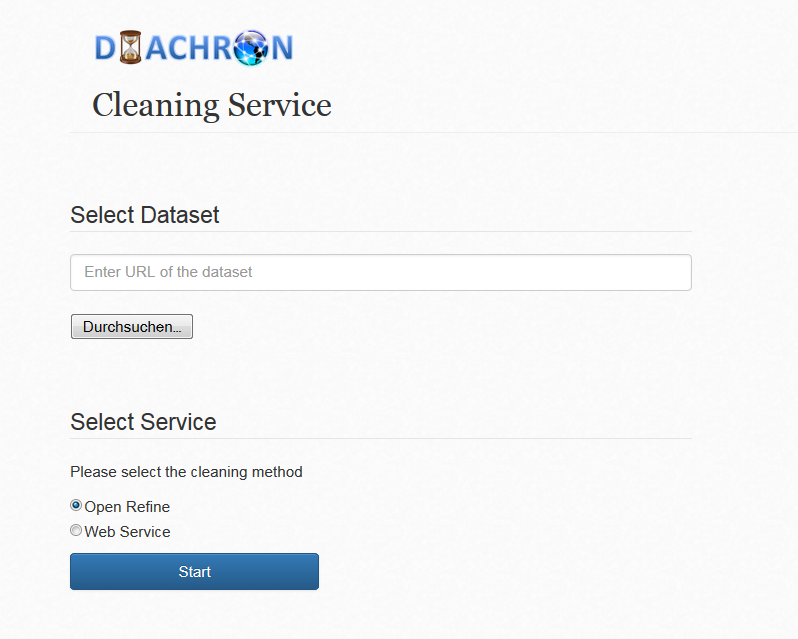
\includegraphics[width=11cm]{figures/CleaningStartPage.PNG}
\caption{User interface of Cleaning Module}
\label{fig:entry}
\end{figure}


\subsection{Cleaning with OpenRefine}
\label{sec:openrefine}

The mains steps of the cleaning workflow using OpenRefine initially described in the Deliverable 3.2~\cite{d3.2} remains unchanged:
\begin{enumerate}
\item Project creation and representation of data set as `subject, predicate, object" table. In contrast to the previous cleaning module version the creation of OpenRefine project
occurs automatically in the back end from the input file defined by the user. 
\item Identification of quality problems. At this step the user define a set of metrics capturing his needs. The metric selection interface slightly changed. The updated version is shown in Figure \ref{fig:metric_selection}.
\item Generation of cleaning suggestions and interactive cleaning. In order to support the user in cleaning process for the UndefinedClass and UndefindedProperty problems we provide the user with concrete examples of classes or properties that could solve this problem. 
\todo{@Ruslan please provide a short description of the used method, reference to used distance metric and a screenshort of the OpenRefine with this suggestion}
\item Export of cleaned data. The list of possible output formats were extended to the most popular formats. The service now supports \texttt{Turtle}, \texttt{RDF/XML}, \texttt{N-Triples}, and \texttt{N3} serialization formats. We also implemented a user interface for this step (Figure \ref{fig:export}).
\end{enumerate}




\begin{figure}[ht!]
\centering
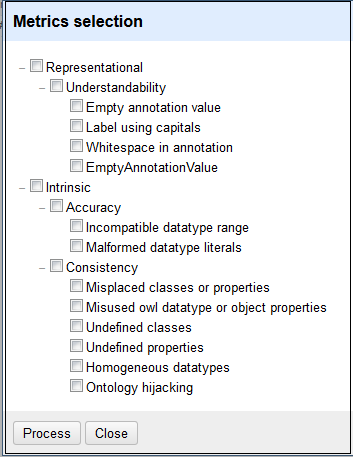
\includegraphics[width=6cm]{figures/MetricSelection.png}
\caption{Metric selection interface}
\label{fig:metric_selection}
\end{figure}



\begin{figure}[ht!]
\centering
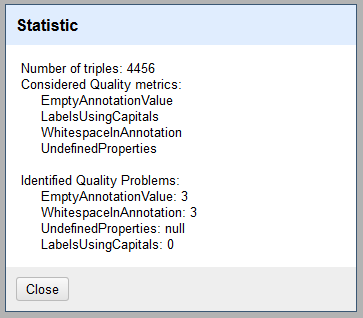
\includegraphics[width=8cm]{figures/statistics.png}
\caption{Cleaning statistics}
\label{fig:statistics}
\end{figure}


\begin{figure}[ht!]
\centering
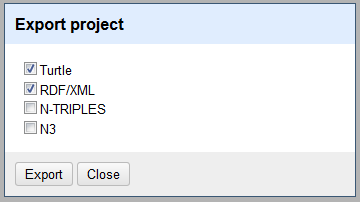
\includegraphics[width=6cm]{figures/export.png}
\caption{Export of cleaned data set in RDF format}
\label{fig:export}
\end{figure}



\todo{@Ruslan please fill the next sections}

\subsection{Technical Documentation}


\subsubsection{Architecture design}
UML diagramm
\subsubsection{Prerequisites}
updates ontologies,
new libraries

\subsubsection{How to install}
In order to use the OpenRefine quality extension you must follow either of the given bellow instructions.
\begin{description}
  \item[Build the extension from source code] \hfill \\
    The extension can be installed from a sketch by building OpenRefine project together with the quality extension.\\
    
  	Step 1. Check out the OpenRefine project from the GitHub repository.\\ 
    \textit{git clone https://github.com/OpenRefine/OpenRefine}\\
  
	Step 2. The extension must be checked out to the directory extension within the OpenRefine root folder.\\
	\textit{git clone https://github.com/diachron/quality-extension.git}\\
	
	Step 3. The two targets for cleaning and building must be add to the ant automation build script the build.xml in the extension directory of OpenRefine. The command \\ \textit{<ant dir="quality-extension/" target="build"/>} must be added to the build target 	and \\ \textit{<ant dir="quality-extension/" target="clean"/>} to the clean target correspondingly.\\
	
	Step 4. The ./refine build command must be run to build the OpenRefine project together with the quality extension.
  
  \item[Install the extension with .zip file] \hfill \\
	The other way of installing the quality extension does not require the build of either quality extension or OpenRefine projects. IN order to have the extension install the few simple following steps must be done.\\
	
	Step 1. Assume that the OpenRefine project is already installed in a local machine.\\
	
	Step 2. Run the OpenRefine and browse to the workspace directory by clicking at the link at the bottom of the project list.\\
	
	Step 3. Download the quality-extension.zip file from the quality extension repository and extract into the "extension" directory in the workspace directory.\\
	
	Step 4. Restart OpenRefine.

\end{description}

\subsubsection{How to run}
\begin{description}
\item[Linux]\hfill \\
The OpenRefine with the installed extension simply run with the command\\
\textit{./refine} at localhost:3333\\
or when specific port and address should be provided\\
\textit{./refine -i 0.0.0.0 -p 3333}
\end{description}

\subsubsection{Integration of new metrics}
The OpenRefine extension can easily be extended with new quality metrics.
To have a metric fully integrated in the extension a developer would have to follow the next steps.

\begin{itemize}
	\item A new metric class must be created in the "com.google.refine.quality.metrics" package and extend the abstract class \texttt{AbstractQualityMetric} by providing the implementation of its abstract methods. The current implementation provides minimal functionality enough to use the metric within the extension. 
	
	Optionally, the metric can be enriched with a specific implementation	 of a related quality problem by extending \texttt{QualityProblem} class located in the "com.google.refine.quality.problems" package. The other improvement to the metric and quality problem pair would be enabling the auto cleaning functionality. It would take place after simple implementation of the \texttt{AutoCleanable} interface which has a single abstract method \textit{getCleanedStatement} with the Jena Statement return value.
	
	\item To enable the quality metric in the OpenRefine extension it must be added to a JSON structure in the JavaScript file in a form of a nested JSON document. For instance, \{"LabelsUsingCapitals" : "Label using capitals"\}, the key of a document must be the precise name of the new metric class. The file can be found by following the path "./module/scripts/metrics-dialog.js".
\end{itemize}

The above steps are enough to integrate the metric in the extension. An instance of the new metric class created dynamically using suing reflection mechanism. The new employed approach facilitates declaration of new metrics, improves maintainability and readability of code. 

%%% Local Variables: 
%%% mode: latex
%%% TeX-master: "D3.2"
%%% End: 
